\documentclass[11pt]{article}

\usepackage{fullpage, graphicx, xcolor, wrapfig}

\graphicspath{{img}}


\begin{document}

\title{ARM Checkpoint... }
\author{Bartłomiej Cieślar, Jordan Hall, Ioana Mihăilescu and Oliver Killane}
\date{27/05/2021}

\maketitle

\section{Group Organisation}
    As the emulator and assembler are separate programs, that can be tested and implemented independently, we made a group decision to develop them in parallel.
    \begin{center}
        \begin{tabular}{ r | l }
            \textbf{Emulator} & \textbf{Assembler} \\
            Ioana \& Oliver & Bartłomiej \& Jordan \\
        \end{tabular}
    \end{center}
    \begin{center}
        \begin{tabular}{r l}
            Daily Standups & To bring up any issues with eachother's code, decide what to work on for the day. \\
            Status Diagram & Each function given a rating determining progress status. (\textcolor{red}{todo}/\textcolor{orange}{implemented}/\textcolor{green}{tested}) \\
            Merge Requests & New features done in separate branches, then merged into \textbf{emulate} to allow for reviews. \\
            Pair programming & Live on call, and with VSCode LiveShare to reduce bug incidence. \\
            Unit Tests & Create unit tests for separable functions as they are implemented. \\
        \end{tabular}
    \end{center}
    \subsection*{Development Cycle}
        \begin{center}
            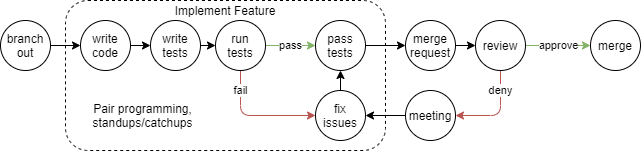
\includegraphics[scale=0.7]{development cycle}
        \end{center}

\section{Implementation Strategies}
    \subsection*{Project Status}
        \begin{center}
            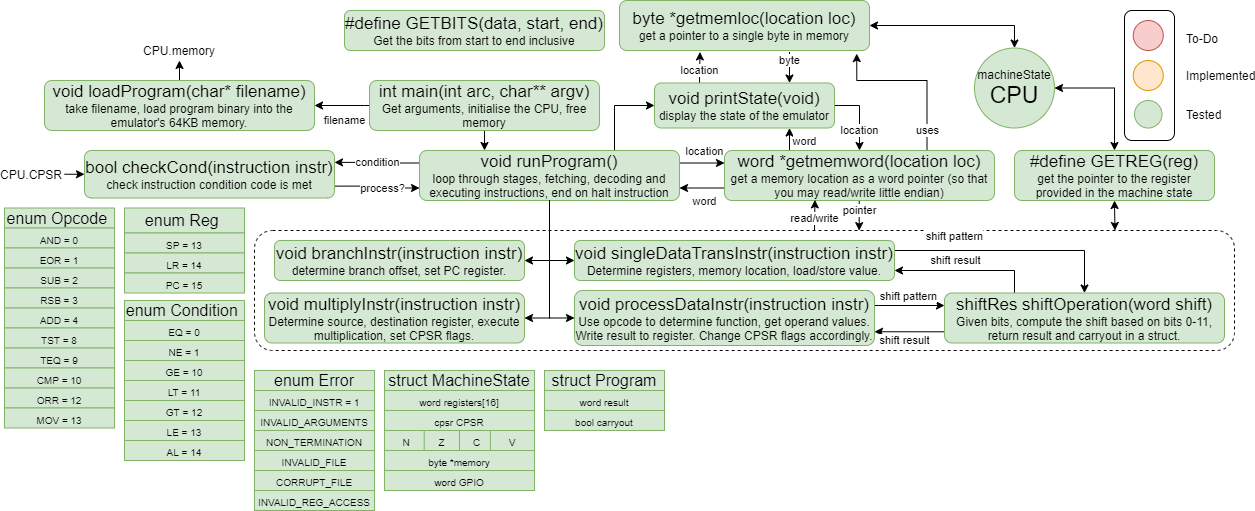
\includegraphics[scale = 0.4]{project status}
        \end{center}
    



\end{document}
